\subsection{Variations of Hidden Markov Models}
\label{subsec:HHMM}

Hidden Markov models rely on several assumptions that are often violated in real-world applications. For example, high-frequency data often violates the assumption that the underlying state process of an HMM is time-homogeneous %, and that the observations are independent when conditioned on the hidden state process 
\citep{Sidrow:2021}. As such, researchers have introduced several variations, such as incorporating covariates into the transition probability matrix $\Gamma$ to account for changing dynamics in the transition matrix \citep{McClintock:2018}. In addition, if a sequence of observations displays multi-scale dependence structure, then it may be more appropriate to use a \textit{hierarchical} hidden Markov model, or HHMM \citep{Barajas:2017,Adam:2019,Sidrow:2021}. Hierarchical HMMs are useful because they capture dependence structures of the hidden process on multiple time scales. There are many different particular ways to define a Hierarchical HMM, such as the formulations in \citet{Barajas:2017}, \citet{Adam:2019}, and \citet{Sidrow:2021}. As presented here, Hierarchical HMMs involve some coarse-scale hidden process that evolves over time. While the coarse-scale state remains in the same state, a fine-scale hidden process evolves simultaneously. Observations are then generated according to a distribution that depends jointly on both the hidden coarse-scale state and the hidden fine-scale state. However, once the coarse-scale process changes states, the fine-scale process restarts and evolves depending upon that new coarse-scale state.

The parameters of an HHMM are defined to enforce this hierarchical structure for the hidden Markov chain. In particular, define a coarse-scale Markov chain $\{X^{(c)}_t\}_{t=1}^T$ parameterized by a pre-determined number of coarse-scale hidden states $N^{(c)} \in \bbN$, a coarse-scale initial distribution $\delta^{(c)} \in \bbR^{N^{(c)}}$ and coarse-scale probability transition matrix $\boldsymbol{\Gamma}^{(c)} \in \bbR^{{N^{(c)}} \times {N^{(c)}}}$. For each coarse-scale state $i$, we yet define another fine-scale Markov chain with states $X^{(f)}_t$ whose length is randomly determined by the dwell time of the coarse-scale Markov chain in state $i$. The $i^{th}$ fine-scale Markov chain is parameterized by a pre-determined number of fine-scale states $N^{(f,i)} \in \bbN$. It also has initial distribution $\delta^{(f,i)} \in \bbR^{N^{(f,i)}}$, and a fine-scale transition probability matrix $\boldsymbol{\Gamma}^{(f,i)} \in \bbR^{N^{(f,i)} \times N^{(f,i)}}$. In summary, 
%
\begin{gather}
    \delta^{(c,i)} = \bbP\left( X_1^{(c)} = i \right) \qquad 
    \Gamma^{(c,i,j)} = \bbP\left( X_{t+1}^{(c)} = j | X_{t}^{(c)} = i \right) \\
    %
    \delta^{(f,i,i')} = \bbP\left( X_{t+1}^{(f)} = i' | X_{t}^{(c)} \neq i, X_{t+1}^{(c)} = i \right) \qquad 
    \Gamma^{(f,i,i',j')} = \bbP\left( X_{t+1}^{(f)} = j' | X_{t}^{(f)} = i', X_{t}^{(c)} = i, X_{t+1}^{(c)} = i \right).
\end{gather}
%
Define the matrix $\boldsymbol{\Pi}^{(f,i)}$ as an $N^{(f,i)} \times N^{(f,i)}$ matrix with identical row entries $\delta^{(f,i)}$. Using this parameterization, the set of pairs $\{(X^{(c)}_t,X^{(f)}_t)\}_{t=1}^T$ is itself Markov chain. It has a total of $N \equiv \sum_{i=1}^{N^{(c)}} N^{(f,i)}$ hidden states, a global initial distribution of
%
\begin{equation} 
\boldsymbol{\delta} = 
\begin{pmatrix}
\delta^{(c,1)}\boldsymbol{\delta}^{(f,1)} & \delta^{(c,2)}\boldsymbol{\delta}^{(f,2)}    & \cdots & \delta^{(c,N^{(c)})}\boldsymbol{\delta}^{(f,N^{(c)})}
\end{pmatrix},
\label{eqn:global_delta}
\end{equation}
%
and a global probability transition matrix of %\textcolor{red}{I stole this from Vianey}:
%
\begin{equation} 
\boldsymbol{\Gamma} = 
\begin{pmatrix}
\Gamma^{(c,1,1)}\boldsymbol{\Gamma}^{(f,1)}     & \Gamma^{(c,1,2)} \boldsymbol{\Pi}^{(f,2)}     & \cdots & \Gamma^{(c,1,N^{(c)})}\boldsymbol{\Pi}^{(f,N^{(c)})}  \cr
\Gamma^{(c,2,1)}\boldsymbol{\Pi}^{(f,1)} & \Gamma^{(c,2,2)} \boldsymbol{\Gamma}^{(f,2)}  & \cdots & \Gamma^{(c,2,N^{(c)})}\boldsymbol{\Pi}^{(f,N^{(c)})} \cr
\vdots & \vdots & \ddots & \vdots \cr 
\Gamma^{(c,N^{(c)},1)}\boldsymbol{\Pi}^{(f,1)} & \Gamma^{(c,N^{(c)},2)}\boldsymbol{\Pi}^{(f,2)}      & \cdots & \Gamma^{(c,N^{(c)},N^{(c)})} \boldsymbol{\Gamma}^{(f,N^{(c)})} 
\end{pmatrix}.
\label{exptpm2}
\end{equation}
%
%corresponds to the probability that the initial coarse-scale hidden state is $i$, and $\Gamma^{(c,i,j)}$ corresponds to the probability that the coarse-scale hidden state will transition to coarse-scale state $j$ given that the current coarse-scale state is $i$. Further, $\delta^{(f,i,i')}$ corresponds to the probability that the initial fine-scale hidden state is $i'$ after transitioning to state $i$ from another state. Finally, $\Gamma^{(f,i,i',j')}$ corresponds to the probability that the fine-scale hidden state will transition to state $j'$ given that the current coarse-scale state is $i$ and the current fine-scale state is $i'$.
%
%Namely, $\delta^{(c,i)} = \bbP\left(X_1^{(c)}\right)$ corresponds to the probability that the initial coarse-scale hidden state is $i$, and $\Gamma^{(c,i,j)}$ corresponds to the probability that the coarse-scale hidden state will transition to coarse-scale state $j$ given that the current coarse-scale state is $i$. Further, $\delta^{(f,i,i')}$ corresponds to the probability that the initial fine-scale hidden state is $i'$ after transitioning to state $i$ from another state. Finally, $\Gamma^{(f,i,i',j')}$ corresponds to the probability that the fine-scale hidden state will transition to state $j'$ given that the current coarse-scale state is $i$ and the current fine-scale state is $i'$.
%
The transition probability matrix $\boldsymbol{\Gamma}$ and initial distribution $\boldsymbol{\delta}$ of a hierarchical HMM is simply a more restricted version of the same parameters for a standard HMM. A visualization of a hierarchical Markov chain with $N^{(c)} = 2$ and $N^{(f,1)} = N^{(f,2)} = 2$ is shown in Figure (\ref{fig:HHMM}).
%
\begin{figure}
    \centering
    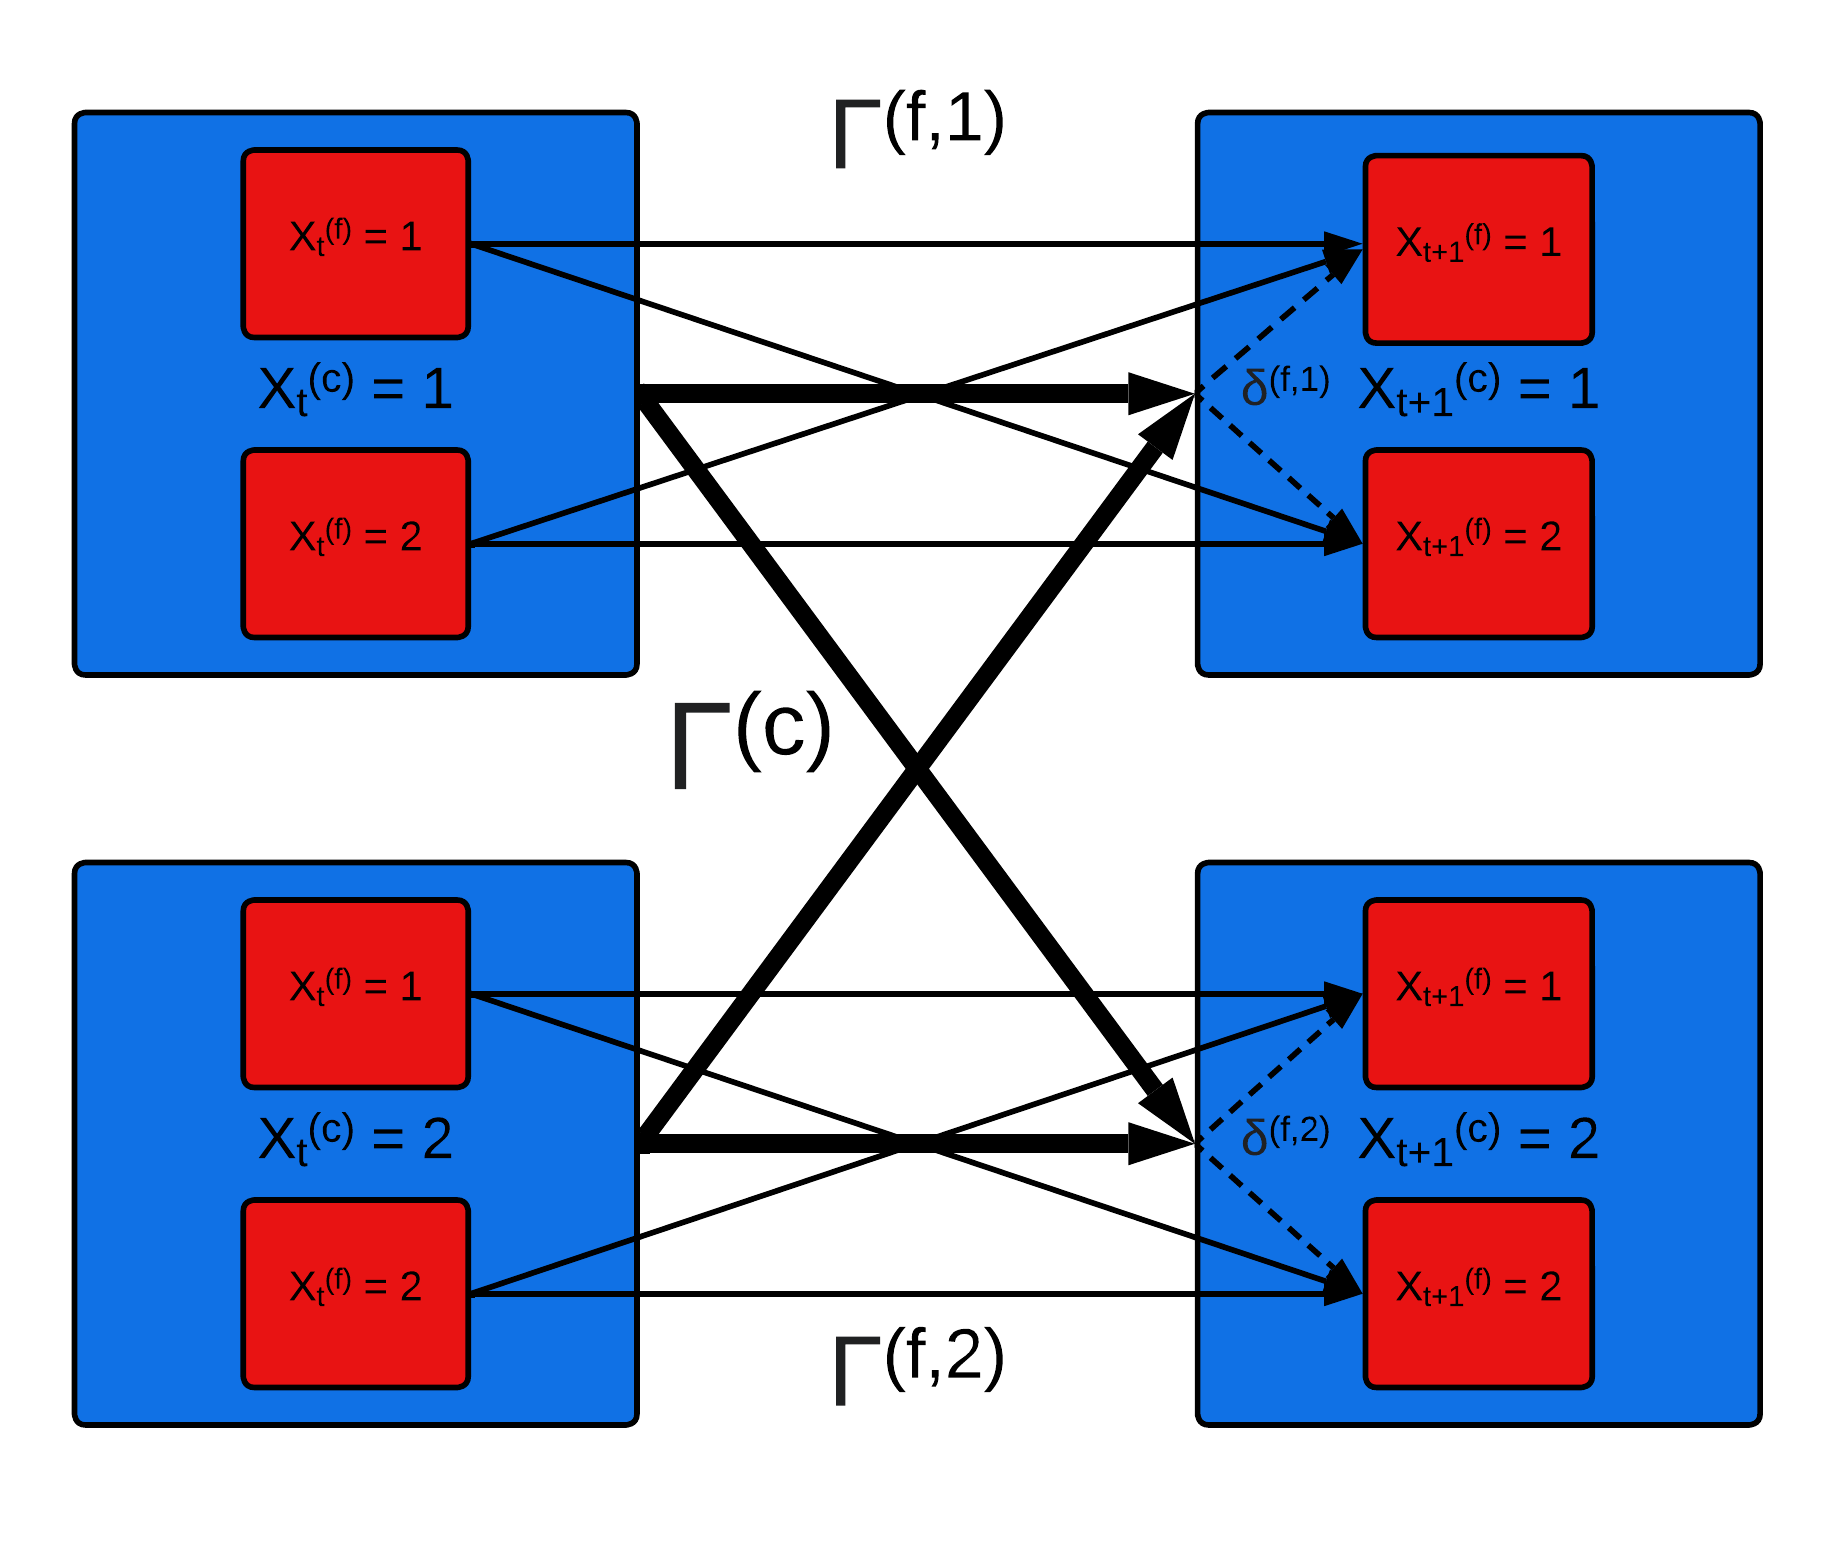
\includegraphics{plt/HHMM.png}
    \caption{Visualization of the underlying Markov chain for a hierarchical HMM with $N^{(c)} = 2$ and $N^{(f,1)} = N^{(f,2)} = 2$. Solid thick lines correspond to entries of $\boldsymbol{\Gamma}^{(c)}$. Solid thin lines correspond to entries of $\boldsymbol{\Gamma}^{(f,i)}$ for $i = 1,2$, which describes the distribution of $X_{t+1}^{(f)}$ if $X^{(c)}_{t} = X^{(c)}_{t+1} = i$. Dashed thin lines correspond to entries of $\boldsymbol{\delta}^{(f,i)}$ for $i = 1,2$, which describes the distribution of $X_{t+1}^{(f)}$ if $X^{(c)}_{t} \neq X^{(c)}_{t+1} = i$.}
    \label{fig:HHMM}
\end{figure}

The coarse-scale and fine-scale initial distributions and transition probability matrices are parameterized similarly to Equation (\ref{eqn:reparam}). In particular, $\boldsymbol{\Gamma}^{(c)}$ and $\boldsymbol{\delta}^{(c)}$ are parameterized via $\eta^{(c)}$ as follows:
%
\begin{equation}
    \Gamma^{(c,i,j)}(\eta^{(c)}) = \frac{\exp(\eta^{(c,i,j)})}{\sum_{k=1}^N \exp(\eta^{(c,i,k)})}, \qquad \delta^{(c,i)}(\eta^{(c)}) = \frac{\exp(\eta^{(c,i)})}{\sum_{k=1}^N \exp(\eta^{(c,k)})}
    \label{eqn:reparam_coarse}
\end{equation}
%
Likewise, $\boldsymbol{\Gamma}^{(f,i)}$ and $\delta^{(f,i)}$ are parameterized via $\eta^f$ as follows:
%
\begin{equation}
    \Gamma^{(f,i,i',j')}(\eta^f) = \frac{\exp(\eta^{(f,i,i',j')})}{\sum_{k'=1}^N \exp(\eta^{(f,i,i',k')})}, \qquad \delta^{(f,i,i')}(\eta^{f}) = \frac{\exp(\eta^{(f,i,i')})}{\sum_{k'=1}^N \exp(\eta^{(f,i,k')})}.
    \label{eqn:reparam_fine}
\end{equation}


\begin{algorithm}
\begin{algorithmic}
\If{$\nabla_{\phi} Q^{(k)}(\phi_{k}) < \epsilon$}:
    \State return $\phi_{k}$
\EndIf

\If{using version 1 and $\log p(\bfy;\phi_{k,\ell+1}) \geq \log p(\bfy;\phi_{k})$}:
    \Comment{move to next iteration}
    \State $\phi_{k+1} \gets \phi_{k,\ell}$
    \State $k \gets k+1$
    \State return to step 2
\ElsIf{using version 2 and $Q^*(\phi_{k}) - Q\big(\phi_{k,\ell} ~ \big| ~ \phi_{k}\big) \leq \frac{\zeta + 1}{2} \Big(Q^*(\phi_{k}) - Q \big(\phi_{k} ~ \big| ~ \phi_{k}\big) \Big)$}
    \State $\phi_{k+1} \gets \phi_{k,\ell,M}$
    \State $k \gets k+1$
    \State return to step 2
\Else
    \State $\ell \gets \ell+1$
    \State return to step 4
\EndIf

\end{algorithmic}
\end{algorithm}